% !TEX encoding = UTF-8 Unicode
% XeLaTeX can use any Mac OS X font. See the setromanfont command below.
% Input to XeLaTeX is full Unicode, so Unicode characters can be typed directly into the source.

% The next lines tell TeXShop to typeset with xelatex, and to open and save the source with Unicode encoding.
% They are not necessary to compile the source by default, but they should remain in case this becomes
% relevant in a future version.

%!TEX TS-program = xelatex
\documentclass{book} % Specifies default font size and document class. The "book" class is nice because it lets us use \section and \subsection.

\usepackage[letterpaper, margin=.5in]{geometry} % Draws pages on letter paper.
\usepackage[x11names]{xcolor} % Used for the line separators between entries in the grad/undergrad lists.
\usepackage[none]{hyphenat} % Prevent Hyphenation - all the students' thank-you messages look terrible without this :)
\usepackage{array} % Used for the Social Media table
\newcolumntype{L}[1]{>{\raggedright\let\newline\\\arraybackslash\hspace{0pt}}m{#1}}
\newcommand{\mystrut}{\rule[-8pt]{0pt}{20pt}}
\newcommand{\mystruts}{\rule[-8pt]{0pt}{36pt}}

% The rest of the packages don't require any special options, so they're grouped together here.
% graphicx and titlepic are for placing the seal image on the cover page. multicol creates columns and is used here on pages and in tables. caption allows us to make nice looking titles for the tables. fontspec lets us pick Helvetica Neue as main font. csvsimple reads and formats student data from .csv files.
\usepackage{graphicx, multicol, caption, titlepic, fontspec, csvsimple, multirow, longtable}

\setmainfont{Helvetica Neue}[Scale=1.25] % Use Helvetica Neue because it's CU Boulder's brand font.

% This section defines the title page. There is no "author" or "title," but it ends up looking exactly how we wanted it anyway.
\title{\Huge{Department of Department Name \\ University of University Name}}
\author{\LARGE{Commencement Recognition Ceremony}}
\date{\LARGE{May 10th, 2020}}
\titlepic{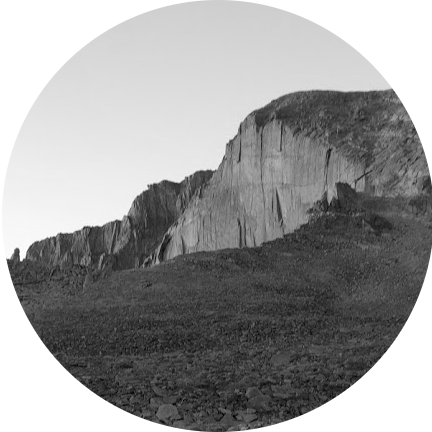
\includegraphics[width=4in]{assets/bitmap.png}} % University seals look very nice on the front of this document, for github, I've uploaded a picture of Longs Peak from the Keyhole route.

\begin{document}
\maketitle

% Schedule and Event Details
%---------------------------
\section*{Schedule of Events} % \section{ } will add numbers to the sections. The asterisk in \section*{ } prevents the number from being added automatically.
  \begin{table}[htp]
  % Options [h], [t], and [p] specify location of the table in the doc. h means here, t means top, and p means (float on) page. [!] may be used to override other formatting (from the document class, for example). There is an example of this usage under "Faculty & Research Interests." The order of the options in the square brackets does not matter.
    \begin{tabular}{l|l}
    % {l|l} is two lowercase "L" characters with a pipe/vertical bar (|) in between. The pipe creates a vertical line between columns, which are separated by &. "l" specifies that each cell is left-aligned. c and r (center and right) can also be used in this context, e.g. {r|c|l} for three columns aligned right, center, and left.
Refreshments Served in Recreation Center Lobby & 9:00am\\
Seating & 9:50am\\
Introduction by Chair - Dr. Crista Trambles & 10:00am\\
Commencement Address - Dr. Claud Ahn & 10:15am\\
Awards Recognition & 10:30am\\
Degree Recognition & 10:40am\\
Closing Remarks/ Departure & 11:40am - 12:00pm

  \end{tabular}
  \end{table}
\section*{Awards} % Sections and subsections are automatically bolded and enlarged in the "book" document class.
\subsection*{TA Award}
Effie Olin
%Enable for semesters when we have these awards
\subsection*{Excellence in Teaching Awards}
Gracie Reitz $\cdot$ Graig Victorino  $\cdot$ Drucilla Mcclary $\cdot$ Kenyetta Voges $\cdot$ Ashanti Stackhouse $\cdot$ Guy Dilorenzo
% $\cdot$ is the raised dot separating the names. It has to be called in "math mode" which is why it's surrounded by $$.
\subsection*{Endowment Recipients}
Mirella Jacobus $\cdot$ Gwyn Zeck $\cdot$ Leslee Wilkinson $\cdot$ Marshall Pauley $\cdot$ Adriana Session $\cdot$ Zola Pettigrew
%\subsection*{Biology Club Award}

%Torrey Davis

\begin{figure}[b]

\section*{Social Media}
% This is a section for social stuff
We would love to have you stay connected with our department! Connect with current students and alumni on our social channels:
\smallskip
  % Line separator
  \begin{center}
 \begin{tabular}{ m{1cm} m{3cm} m{1cm} m{3cm} m{1cm} m{3cm} }
  
\includegraphics[width=.5in]{assets/fb-icon.png} & Facebook Department Name & 
\includegraphics[width=.5in]{assets/ig-icon.png} & Instagram @example & 
\includegraphics[width=.5in]{assets/ln-icon.png} & LinkedIn Group\\
  \smallskip \\
 \end{tabular}

 \em https://www.example.com/department/social-media
  \end{center}
\end{figure}
\clearpage

 % Ensures that nothing else is written or drawn on this page. Subsequent content begins on a fresh page.
%---------------------------
% Test csv page for faculty.
% \clearpage % We could use the longtabu environment to make this into one long table over multiple pages instead of having two tables.

%\section*{\LARGE{EBIO Department Faculty \& Research Interests}}
%http://texdoc.net/texmf-dist/doc/latex/multirow/multirow.pdf - super helpful
%https://tex.stackexchange.com/questions/72945/how-to-merge-cells-vertically
%---------------------------

% Faculty & Research Interests
%---------------------------
\begin{table}[ht!] % Example of using ! option along with h and t for the table.
{\bfseries\Large{Department Faculty \& Research Interests}}
\\

\begin{tabular}{p{2.5in} p{4.5in}}
% {p{width} p{width}} specifies that the two cells in each row are formatted as paragraphs of specified width; contrast with the above {l|l}-type notation, which will set column widths to be equal to the longest entry in the column (need to check this) and also will not allow newlines within cells.

% Using \newline instead of \\ within the left column cells prevents LaTeX from creating a new table row.
% \newline inside the cell only creates a new line for that one cell. Using \\ \\ at the end of each row leaves a nice space between entries.
% When we want to write "&" in the actual table (or anywhere else in the document), it must be coded with the escape character as "\&".
\textbf{Fernande Wake} \newline Professor & Lorem ipsum dolor sit amet, consectetur adipiscing elit..\\ \\
\textbf{Crista Tramble} \newline Associate Professor & Vestibulum quis purus vulputate, porta quam at, vulputate turpis.\\ \\
\textbf{Yun Mathes} \newline Professor \newline Curator of Science & Sed in urna et magna hendrerit lobortis id et mauris.\\ \\
\textbf{Natalya Boley} \newline Professor and Director, HVAC & Ut et mi venenatis nibh efficitur pretium at non risus..\\ \\
\textbf{Grayce Asbury} \newline Professor & Nullam at ante ut leo consequat pellentesque in et lorem. \\ \\
\textbf{Mica Aden} \newline Assistant Professor & Fusce eget lorem a purus laoreet facilisis id vitae velit. \\ \\
\textbf{Theressa Breton} \newline Associate Professor & Aliquam aliquam arcu sollicitudin urna semper, vitae maximus ex ultricies.\\ \\
\textbf{Aleen Dobles } \newline Professor & Curabitur rhoncus odio eu molestie sagittis.\\ \\
\textbf{Paulita Nesby} \newline Associate Professor & Pellentesque sit amet sem semper, interdum leo vitae, placerat neque.\\ \\
\textbf{Rita Rick} \newline Assistant Professor & Morbi bibendum tortor at arcu convallis maximus. \\ \\
\textbf{Lara Osterberg} \newline Professor & Pellentesque ac leo hendrerit, aliquet est eu, condimentum nisi.\\ \\
\textbf{Fabiola Wegener} \newline Associate Professor & Cras condimentum erat ac nulla mollis, ut consectetur ligula suscipit. \\ \\
\textbf{Timmy Vien} \newline Professor & In faucibus dolor eu nibh pretium, eget pulvinar lorem suscipit.\\ \\
\textbf{Claud Ahn} \newline Assistant Professor & Mauris rhoncus urna ac erat dictum, a semper lorem maximus.\\ \\
\textbf{Kristle Dobbin} \newline Professor \newline Curator of Plants & Curabitur vestibulum velit et mi tincidunt, eu cursus neque porta.\\ \\
\textbf{Selena Staples} \newline Professor & Aenean accumsan turpis vitae lorem varius, ut aliquam neque fermentum.\\ \\
\textbf{Laureen Wotring} \newline Assistant Professor \newline Curator of Lobsters & Maecenas sed tortor semper, mattis lorem sed, molestie nisl.\\ \\

\end{tabular}
\end{table}

\clearpage % We could use the longtabu environment to make this into one long table over multiple pages instead of having two tables.

\begin{table}[ht!]
%\caption*{\bfseries\Large{EBIO Department Faculty \& Research Interests, cont'd}}
\begin{tabular}{p{2.5in} p{4.5in}}

\textbf{Tammy Maul} \newline Professor & Praesent a dolor vel turpis tincidunt tempor eu at mi.\\ \\
\textbf{Nichole Girardin} \newline Associate Professor \newline Curator of Fish & Proin pretium elit non massa tristique, a eleifend sem cursus.\\ \\
\textbf{Ethyl Weidemann} \newline Associate Professor & Quisque a augue quis enim gravida luctus.\\ \\
\textbf{Emerson Boltz} \newline Associate Professor & Phasellus sollicitudin tellus a turpis fermentum consectetur.\\ \\
\textbf{Thi Hoyte} \newline Associate Professor & Quisque eget quam ultricies, mattis erat at, dictum lacus..\\ \\
\textbf{Chase Forgione} \newline Professor & In eget metus eget ex porttitor venenatis nec nec enim.\\ \\
\textbf{Salina Ellenburg} \newline Assistant Professor & Phasellus nec eros et turpis iaculis tempus fringilla in odio.\\ \\
\textbf{Nestor Mcree} \newline Assistant Professor & Donec non justo in ipsum porttitor convallis.\\ \\
\textbf{Jenise Broad} \newline Associate Professor & Pellentesque blandit nunc vitae lorem posuere, hendrerit convallis est cursus.\\ \\
\textbf{Steven K. Schmidt} \newline Professor & Sed rutrum augue vel arcu lobortis fringilla.\\ \\
\textbf{Minerva Molinaro} \newline Professor & Aenean in dolor ac ex viverra dignissim.\\ \\
\textbf{Marni Poteat} \newline Associate Professor & Duis dignissim mi sit amet velit consectetur, at commodo mauris imperdiet.\\ \\
\textbf{Tessie Able} \newline Associate Professor &  Pellentesque aliquet neque quis pulvinar eleifend.\\ \\
\textbf{Jolanda Schilling} \newline Professor & Pellentesque lacinia nulla vitae mauris porttitor euismod.\\ \\
\textbf{Sophie Carr} \newline Assistant Professor & Proin consequat quam id turpis ultricies aliquet.\\ \\
\textbf{Lasonya Ledoux} \newline Assistant Professor \newline Curator of Frogs & Sed ut lectus placerat ipsum bibendum blandit quis sed ligula.\\ \\
\textbf{Hugh Lando} \newline Professor & Fusce commodo tellus elementum, feugiat risus vitae, ornare est.

\end{tabular}
\caption*{\textit{http://www.example.com/department/professors}}
\end{table}

\clearpage
%---------------------------
%---------------------------
% Begin student data
%---------------------------
% Graduates
%---------------------------
\clearpage
\section*{\LARGE{PhD and MA Graduates}}
% This section and the following student sections read data from external .csv files and format them according to the specified macros.
% The .csv will need to be formatted carefully. Entries that contain commas and certain other characters need to be enclosed in curly braces { }.
% If you prepare a .csv in that manner (using TextEdit) and then open it in Microsoft Excel, it will ruin the formatting so it won't work when TeX compiles it.
\csvreader{data/graduate-students.csv}{3=\name, 4=\status, 5=\advisor, 6=\dissertation, 7=\thesis, 8=\thanks}
% Here, the .csv is called GradListFinal2. It is (should be) in the same directory as this .tex file. The macros \name, \status, etc. are aliases for the columns in the .csv.
  {\subsection*{\name\hfill\status} % \hfill fills in any white space between \name, the right edge (margin) of the page, and \status, so that \status is against the margin.
  \textit{\dissertation\thesis} \\  % Italicize dissertation/thesis titles. Since no student has both a dissertation and a thesis, this will always print ONLY one or the other, but not both. If a student did have both, this would need to be rewritten.
  Advisor(s): \advisor\\ \\
  \thanks % You're welcome!

  % Line separator
  \begin{center} % Horizontally centers the line we're about to draw using \rule.
  \textcolor{lightgray}{\rule{.25cm}{0.15mm}} % \textcolor{color}{\rule{line length}{line width}}
  % The color can be specified in plain English. The xcolor package should allow us to use some complicated color names, but some of them did not seem to work.
  \end{center}
  } % End of what csvreader is reading.
%---------------------------
\clearpage
%---------------------------
% Undergraduates
%---------------------------
\section*{\LARGE{Undergraduates - Honors Theses}}
% This section uses the same formatting as "PhD and MA Graduates," but the data is imported from a different .csv containing only the names of undergraduates who received honors designations, along with their thesis titles and advisor names.
% Undergraduates with honors and thesis titles
\csvreader{data/undergraduate-honors.csv}{1=\name, 2=\thesis, 3=\advisor, 4=\honors,}
  {\subsection*{\name\hfill\textit{\small\honors}} % \textit{\small\honors} outputs the honors designation in a smaller font point, italicized.
  Thesis Title: \textit{\thesis}\\
  Advisor: \advisor\\
  \begin{center}
  \textcolor{lightgray}{\rule{.25cm}{0.15mm}}
  \end{center}
  }
%---------------------------
% All undergraduates
%---------------------------
\clearpage % We could use the longtable environment to make this into one long table over multiple pages instead of having two tables.
\section*{\LARGE{Undergraduates}}
% This section lists all undergrads, including the ones who earned honors, but only lists their names, honors designation (where applicable), and thank-you message. The .csv we used for this version (which was a third, separate .csv from the previous two) also included three extra beginning columns that were unused as macros.
\begin{multicols}{2} % To save space, this list is done as two columns of text.
\csvreader{data/undergraduate-students.csv}{3=\name, 5=\thanks, 6=\honors}
  {\subsection*{\name\hfill\textit{\small\honors}}
  \thanks

  % Line separator
  \begin{center}
  \textcolor{lightgray}{\rule{.25cm}{0.15mm}} % This line is half the length of the others since we're now writing in two columns.
  \end{center}
  }
\end{multicols}
% End student data
%---------------------------
\end{document}
